% Tanpa Animasi
%\documentclass[aspectratio=169,handout]{beamer}

% Animasi
\documentclass[aspectratio=169]{beamer}

% Pdf Untuk di Print
%\usepackage{pgfpages}
%\pgfpagesuselayout{2 on 1}[a4paper, border shrink=5mm]

\hypersetup{pdfpagemode=FullScreen} %agar pdf auto fullscreen

\setbeamertemplate{frametitle continuation}{} %untuk menghilangkan penomoran pada allowframebreaks
\usetheme{Madrid}
\usepackage[indonesian]{babel}

% Perlengkapan flowchart
\usepackage{tikz}
\usetikzlibrary{shapes.geometric, arrows}

% Pemenggalan Kata
\usepackage[none]{hyphenat} %tanpa pemenggalan kata
\sloppy %teks rapi

\usepackage{ragged2e}
\usepackage{hyperref}

\usepackage{caption}
\usepackage{subcaption}

%\setbeamercovered{transparent} %agar teks transparan

% Perlengkapan pada table
\usepackage{colortbl} %untuk color table
\usepackage{adjustbox} %agar table pas di halaman (tidak lebih)
\usepackage{longtable} %Untuk membuat table lebih panjang
\usepackage{multirow}

% Identitas
\title[\textit{Multiple Travelling Salesman Problem}]{PENERAPAN K-MEANS DAN ALGORITMA GENETIKA UNTUK
MENYELESAIKAN MTSP}
\subtitle{(Studi Kasus Pada Perjalanan Menuju Seluruh SMA di Kabupaten Probolinggo)}
\author{Muhammad Faiz Nailun Ni'am}
\institute[PMAT UNUJA]{Pendidikan Matematika \\Universitas Nurul Jadid}
\date{27 Juli 2022}
\titlegraphic{
\includegraphics[width=2cm]{lain-lain/logo}}

\begin{document}
\begin{frame}
\titlepage
\end{frame}

\begin{frame}
\frametitle{Daftar Isi}
\tableofcontents
\end{frame}

\section{Latar Belakang}
\begin{frame}
\frametitle{Pendahuluan}
\begin{block}{Latar Belakang}
\begin{figure}[H]
\centering
%Definisi
\tikzstyle{kotak} = [rectangle, minimum height=2cm, text width=3cm, text centered, draw=black, fill=blue!30]
\tikzstyle{garis} = [thick,->,>=stealth]
%Gambar
\begin{tikzpicture}
\scriptsize
\onslide<1-> \node (1) [kotak] {Beberapa lembaga di Kabupaten Probolinggo mengadakan acara seperti olimpiade, kompetisi, dan lain-lain};
\onslide<2-> \node (2) [kotak, right of=1, xshift=+2.8cm]{Dibutuhkan penyebaran barang berupa poster, undangan, dan surat selebaran ke beberapa sekolah};
\onslide<3-> \node (3) [kotak, right of=2, xshift=+2.8cm]{Dibutuhkan pencarian rute terdekat untuk menuju ke lokasi-lokasi tersebut};
\onslide<4-> \node (4) [kotak, right of=3, xshift=+2.8cm]{Permasalahan pencarian rute tersebut disebut \textit{Traveling Salesman Problem} (TSP)};
\onslide<5-> \node (5) [kotak, below of=4, yshift=-1.5cm]{Gabungan dari beberapa permasalahan TSP disebut \textit{Multiple Traveling Salesman Problem} (MTSP)};
\onslide<6-> \node (6) [kotak, left of=5, xshift=-2.8cm]{Menurut beberapa peneliti sebelumnya algoritma genetika cukup efektif untuk skala kota kecil};
\onslide<7-> \node (7) [kotak, left of=6, xshift=-2.8cm]{dan algoritma $k$-means dapat digunakan untuk mengklaster};
\onslide<8-> \node (8) [kotak, left of=7, xshift=-2.8cm]{Dalam penelitian ini akan digunakan algoritma genetika dan $k$-means untuk menyelesaikan MTSP};

\onslide<1-> \draw [garis] (1) -- (2);
\onslide<2-> \draw [garis] (2) -- (3);
\onslide<3-> \draw [garis] (3) -- (4);
\onslide<4-> \draw [garis] (4) -- (5);
\onslide<5-> \draw [garis] (5) -- (6);
\onslide<6-> \draw [garis] (6) -- (7);
\onslide<7-> \draw [garis] (7) -- (8);
\end{tikzpicture}
\end{figure}
\end{block}
\end{frame}
\section{Tujuan Penelitian}
\begin{frame}
\frametitle{Tujuan Penelitian}
\begin{block}{Tujuan Penelitian}
\begin{enumerate}
\item Mengetahui cara menemukan solusi \textit{Multiple Travelling Salesman Problem} menggunakan algoritma genetika dan $k$-means.
\item Menemukan solusi pembagian klaster dan urutan jalur terdekat menuju seluruh SMA di Kabupaten Probolinggo.
\end{enumerate}
\end{block}
\end{frame}
\section{Batasan Masalah}
\begin{frame}
\frametitle{Batasan Masalah}

\begin{block}<1->{Batasan Masalah}
\begin{enumerate}
\item Menggunakan 1 titik asal dan setiap \textit{salesman} akan berangkat dan kembali pada titik kota yang sama.
\item Titik-titik tujuan adalah koordinat lokasi 75 SMA di Kabupaten Probolinggo baik negeri maupun swasta.
\item Tidak ada prioritas sekolah mana saja yang dilalui terlebih dahulu.
\end{enumerate}
\end{block}
\begin{block}<2->{Asumsi}
\begin{enumerate}
\item Setiap titik tujuan diasumsikan selalu terhubung dan berjalan lurus.
\item Titik kumpul menggunakan koordinat rata-rata dari semua
\item Jarak yang digunakan adalah jarak \textit{Euclidean distance} (Jarak garis lurus antara 2 titik)
\end{enumerate}
\end{block}
\end{frame}
\begin{frame}
\frametitle{Penelitian Terdahulu}
\begin{block}<1->{\textit{Applying K-means and Genetic Algorithm for Solving MTSP}}
Membahas tentang persilangan jalur antara tiap \textit{salesman} yang dapat dihindari dengan menggunakan algoritma genetika dan \textit{k}-means yang dapat meminimalisir terjadinya tabrakan antara \textit{salesman}.
\end{block}

\begin{block}<2->{Optimasi \textit{Multiple Travelling Salesman Problem} (M-TSP) pada Penentuan Rute Optimal Penjemputan Penumpang \textit{Travel} Menggunakan Algoritme Genetika}
Membahas permasalahan \textit{salesman} yang akan berangkat dari kantor \textit{travel} menuju ke alamat penjemputan masing-masing penumpang. Pada permasalahan tersebut menggunakan representasi permutasi, proses reproduksi \textit{crossover}, mutasi, dan seleksi.
\end{block}

\begin{block}<3->{Penyelesaian \textit{Multitraveling Salesman Problem} dengan Algoritma Genetika}
Membahas kinerja algoritma genetika berdasarkan jarak minimum dan waktu pemrosesan yang diperlukan untuk 10 kali pengulangan untuk setiap kombinasi kota penjual.
\end{block}
\end{frame}
\section{Metode Penelitian}
\begin{frame}
\frametitle{Metode Penelitian}
\begin{block}{Tahapan Penelitian}
\begin{figure}[H]
\centering
%Definisi
\tikzstyle{kotak} = [rectangle, minimum height=2cm, text width=3cm, text centered, draw=black, fill=blue!30]
\tikzstyle{garis} = [thick,->,>=stealth]
%Gambar
\begin{tikzpicture}
\scriptsize
\onslide<1-> \node (1) [kotak] {Pengumpulan Data};
\onslide<2-> \node (2) [kotak, right of=1, xshift=+2.8cm]{Pengolahan Data};
\onslide<3-> \node (3) [kotak, right of=2, xshift=+2.8cm]{Analisis};
\onslide<4-> \node (4) [kotak, right of=3, xshift=+2.8cm]{Implementasi};

\onslide<1-> \draw [garis] (1) -- (2);
\onslide<2-> \draw [garis] (2) -- (3);
\onslide<3-> \draw [garis] (3) -- (4);
\end{tikzpicture}
\end{figure}
\end{block}

\begin{block}<5->{Data Penelitian}
Dalam penelitian ini data yang digunakan adalah nama dan koordinat lokasi dari seluruh SMA di Kabupaten Probolinggo yang dikumpulkan dari:

\begin{enumerate}
\item \url{https://referensi.data.kemdikbud.go.id/} (Daftar Nama Sekolah di Kabupaten Probolinggo)
\item \url{https://earth.google.com/} (Koordinat lokasi sekolah)
\end{enumerate}
\end{block}
\end{frame}
\begin{frame}
\frametitle{SMA di Kabupaten Probolinggo}
\begin{figure}
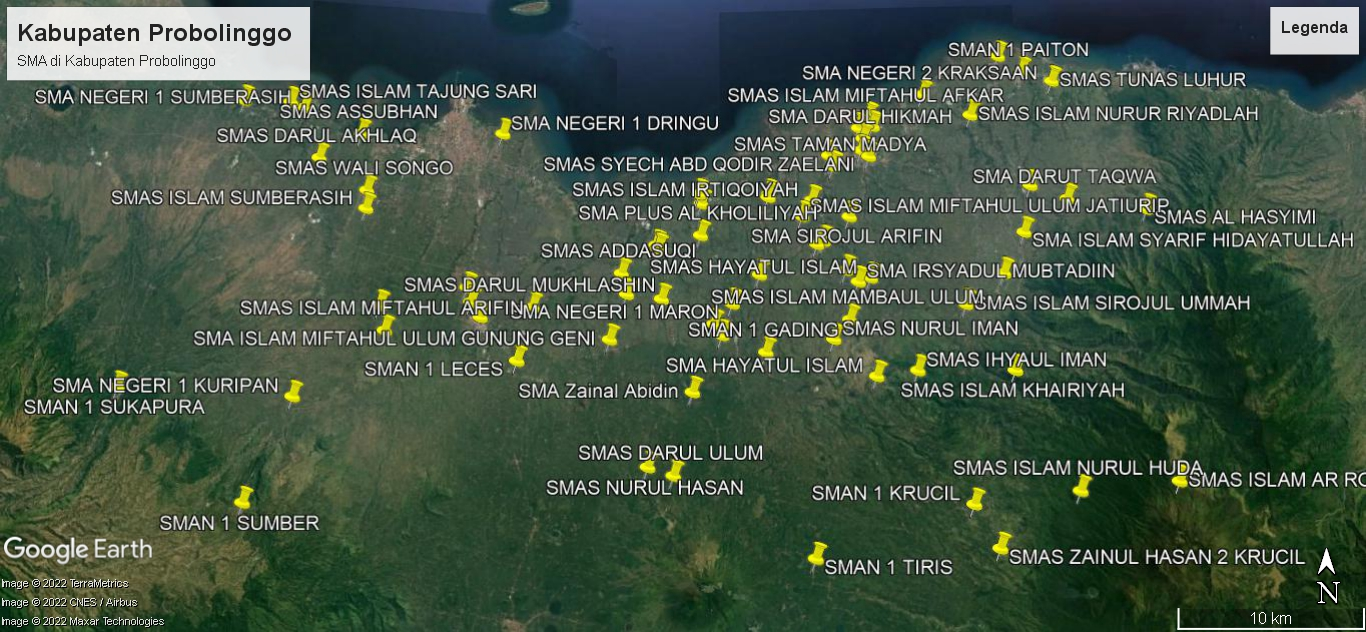
\includegraphics[width=0.8\textwidth]{gambar/Peta SMA}
\caption{75 SMA Negeri dan Swasta di Kabupaten Probolinggo}
\end{figure}
\end{frame}
\section{Jarak \textit{Euclidean distance}}
\begin{frame}
\frametitle{\textit{Euclidean distance}}

\begin{block}<1->{Definisi}
\textit{Euclidean distance} adalah jarak garis lurus antara dua titik.
\end{block}

\begin{block}<2->{Persamaan \textit{Euclidean distance}}
\begin{equation}
d_{ij}=\sqrt{\left( x_j-x_i \right)^{2}+\left( y_j-y_i \right)^{2}}
\end{equation}

Keterangan:
\begin{itemize}
\item $d_{ij}$ adalah nilai jarak pada titik $i$ ke titik $j$
\item $x_i$ dan $y_i$ adalah nilai koordinat $x$ dan $y$ pada titik $i$
\item $x_j$ dan $y_j$ adalah nilai koordinat $x$ dan $y$ pada titik $j$
\end{itemize}
\end{block}

\end{frame}
\section{Alur $K$-means dan Algoritma Genetika}

\begin{frame}
\frametitle{Alur $K$-means dan Algoritma Genetika}
\begin{block}{Algoritma $k$-means}
\begin{figure}[H]
\linespread{1}
\centering
%Definisi
\tikzstyle{bulat} = [rectangle, rounded corners, text width=2cm, minimum height=1cm, minimum width=2cm, text centered, draw=black, fill=red!30]
\tikzstyle{jajargenjang} = [trapezium, trapezium left angle=70, trapezium right angle=110, text width=1.5cm, minimum height=1cm, minimum width=1.5cm, text centered, draw=black, fill=blue!30]
\tikzstyle{kotak} = [rectangle, text width=2.5cm, minimum height=1cm, minimum width=2cm, text centered, draw=black, fill=orange!30]
\tikzstyle{belahketupat} = [diamond, text width=2cm, minimum height=1cm, minimum width=2cm, text centered, draw=black, fill=green!30]
\tikzstyle{garis} = [thick,->,>=stealth]

%Gambar
\begin{tikzpicture}
\onslide<1-> \node (1) [bulat] {Mulai};
\onslide<2-> \node (2) [jajargenjang, below of=1, yshift=-0.8cm]{Dataset, tentukan $n$ klaster};
\onslide<3-> \node (3) [kotak, below of=2, yshift=-1.2cm] {Pilih \textit{centroid} secara acak};
\onslide<4-> \node (4) [kotak, right of=3, xshift=+2.5cm] {Hitung \textit{fitness}};
\onslide<5-> \node (5) [kotak, above of=4, yshift=+2.6cm] {Pengelompokan berdasarkan \textit{fitness} terkecil};
\onslide<6-> \node (6) [kotak, right of=5, xshift=+2.5cm] {Memindahkan \textit{centroid} ke tengah area};
\onslide<7-> \node (7) [belahketupat, below of=6, yshift=-2.6cm]{\textit{Centroid} bergeser?};
\onslide<8-> \node (8) [jajargenjang, right of=7, xshift=+2.5cm] {Hasil $k$-means};
\onslide<9-> \node (9) [bulat, above of=8, yshift=+0.6cm] {Selesai};

\onslide<1-> \draw [garis] (1) -- (2);
\onslide<2-> \draw [garis] (2) -- (3);
\onslide<3-> \draw [garis] (3) -- (4);
\onslide<4-> \draw [garis] (4) -- (5);
\onslide<5-> \draw [garis] (5) -- (6);
\onslide<6-> \draw [garis] (6) -- (7);
\onslide<7-> \draw [garis] (7) -- node[near start, color=black, yshift=+0.5cm]{Ya}(4);
\onslide<7-> \draw [garis] (7) -- node[near start, color=black, yshift=+0.5cm]{Tidak}(8);
\onslide<8-> \draw [garis] (8) -- (9);

\end{tikzpicture}
\end{figure}
\end{block}
\end{frame}


\begin{frame}
\frametitle{Alur $K$-means dan Algoritma Genetika}
\begin{block}{Algoritma genetika}
\begin{figure}[H]
\centering
\linespread{1}
%Definisi
\tikzstyle{bulat} = [rectangle, rounded corners, text width=2cm, minimum height=1cm, minimum width=2cm, text centered, draw=black, fill=red!30]
\tikzstyle{jajargenjang} = [trapezium, trapezium left angle=70, trapezium right angle=110, text width=1.5cm, minimum height=1cm, minimum width=1.5cm, text centered, draw=black, fill=blue!30]
\tikzstyle{kotak} = [rectangle, text width=2cm, minimum height=1cm, minimum width=2cm, text centered, draw=black, fill=orange!30]
\tikzstyle{belahketupat} = [diamond, text width=2cm, minimum height=1cm, minimum width=2cm, text centered, draw=black, fill=green!30]
\tikzstyle{garis} = [thick,->,>=stealth]
%Gambar
\begin{tikzpicture}
\onslide <1-> \node (S) [bulat] {Mulai};
\onslide <2-> \node (in) [jajargenjang, below of=S, yshift=-0.6cm]{Dataset};
\onslide <3-> \node (pop) [kotak, below of=in, yshift=-0.6cm] {Bangkitkan Populasi Awal};
\onslide <4-> \node (fit) [kotak, right of=pop, xshift=+2.5cm] {Hitung \textit{Fitness}};
\onslide <5-> \node (sel) [kotak, above of=fit, yshift=+0.6cm] {Seleksi};
\onslide <6-> \node (cross) [kotak, above of=sel, yshift=+0.6cm] {\textit{Crossover}};
\onslide <7-> \node (mut) [kotak, right of=cross, xshift=+2.5cm] {Mutasi};
\onslide <8-> \node (opt) [belahketupat, below of=mut, yshift=-2.2cm] {Optimal};
\onslide <9-> \node (out) [jajargenjang, right of=opt, xshift=+2cm]{Kromosom Optimal};
\onslide <10-> \node (E) [bulat, above of=out, yshift=+0.6cm] {Selesai};

\onslide <1-> \draw [garis] (S) -- (in);
\onslide <2-> \draw [garis] (in) -- (pop);
\onslide <3-> \draw [garis] (pop) -- (fit);
\onslide <4-> \draw [garis] (fit) -- (sel);
\onslide <5-> \draw [garis] (sel) -- (cross);
\onslide <6-> \draw [garis] (cross) -- (mut);
\onslide <7-> \draw [garis] (mut) -- (opt);
\onslide <8-> \draw [garis] (opt) -- node[near start, color=black, yshift=+0.3cm]{Ya}(out);
\onslide <8-> \draw [garis] (opt) -- node[near start, color=black, yshift=+0.3cm]{Tidak}(fit);
\onslide <9-> \draw [garis] (out) -- (E);
\end{tikzpicture}
\end{figure}
\end{block}
\end{frame}
\section{Hasil}

\begin{frame}
\frametitle{Hasil}
\begin{block}{Total jarak dari tiap pembagian klaster}
\begin{table}[H]
\centering
\footnotesize
\begin{tabular}{ccccc}
\rowcolor[HTML]{4472C4} 
\cellcolor[HTML]{4472C4}{\color[HTML]{FFFFFF} } &
  \cellcolor[HTML]{4472C4}{\color[HTML]{FFFFFF} } &
  \cellcolor[HTML]{4472C4}{\color[HTML]{FFFFFF} } &
  \multicolumn{2}{c}{\cellcolor[HTML]{4472C4}{\color[HTML]{FFFFFF} \textbf{Titik Kumpul}}} \\
\rowcolor[HTML]{4472C4} 
\multirow{-2}{*}{\cellcolor[HTML]{4472C4}{\color[HTML]{FFFFFF} \textbf{Banyak Klaster}}} &
  \multirow{-2}{*}{\cellcolor[HTML]{4472C4}{\color[HTML]{FFFFFF} \textbf{Total Jarak}}} &
  \multirow{-2}{*}{\cellcolor[HTML]{4472C4}{\color[HTML]{FFFFFF} \textbf{Peringkat}}} &
  \cellcolor[HTML]{4472C4}{\color[HTML]{FFFFFF} \textbf{Latitude (X)}} &
  \cellcolor[HTML]{4472C4}{\color[HTML]{FFFFFF} \textbf{Longitude (Y)}} \\
\onslide<2-> 1  & 10,0503  & 10 & -7,8221841 & 113,3570412 \onslide<3-> \\
\rowcolor[HTML]{D9E1F2} 
2  & 6,858777 & 9  & -7,8241236 & 113,3236903 \onslide<4-> \\
3  & 5,599878 & 8  & -7,8219762 & 113,3512877 \onslide<5->\\
\rowcolor[HTML]{D9E1F2} 
4  & 5,010994 & 7  & -7,8215022 & 113,3644199 \onslide<6-> \\
5  & 4,805015 & 6  & -7,828521  & 113,3744846 \onslide<7-> \\
\rowcolor[HTML]{D9E1F2} 
6  & 4,43132  & 3  & -7,8265701 & 113,3475373 \onslide<8-> \\
7  & 4,353295 & 1  & -7,8331118 & 113,3721289 \onslide<9-> \\
\rowcolor[HTML]{D9E1F2} 
8  & 4,398984 & 2  & -7,8358502 & 113,3704048 \onslide<10-> \\
9  & 4,48243  & 4  & -7,8321462 & 113,356253  \onslide<11-> \\
\rowcolor[HTML]{D9E1F2} 
10 & 4,780413 & 5  & -7,8406976 & 113,3665328
\end{tabular}
\end{table}
\end{block}
\end{frame}
\section{Kesimpulan dan Saran}
\begin{frame}
\frametitle{Kesimpulan dan Saran}

\begin{block}<1->{Kesimpulan}
\begin{enumerate}
\item Jalur terpendek menuju seluruh SMA di Kabupaten Probolinggo dapat menggunakan algoritma genetika dan $k$-means dengan pembagian 7 klaster.
\item Jarak yang dihasilkan dengan pembagian klaster tersebut adalah $4,353294644$ satuan koordinat dengan urutan perjalanan sebagaimana tertera pada naskah skripsi.
\end{enumerate}
\end{block}

\begin{block}<2->{Saran}
\begin{enumerate}
\item Mencoba algoritma lain untuk mengetahui metode yang lebih efektif dan untuk mengurangi persilangan jalur antar \textit{salesman}.
\item Menambahkan variabel waktu tempuh, karena dalam penelitian ini hanya variabel jarak saja.
\item Jarak dapat menggunakan jarak asli bukan dengan \textit{Euclidean distance}
\end{enumerate}
\end{block}
\end{frame}
\end{document}